% Options for packages loaded elsewhere
\PassOptionsToPackage{unicode}{hyperref}
\PassOptionsToPackage{hyphens}{url}
%
\documentclass[
]{article}
\usepackage{amsmath,amssymb}
\usepackage{iftex}
\ifPDFTeX
  \usepackage[T1]{fontenc}
  \usepackage[utf8]{inputenc}
  \usepackage{textcomp} % provide euro and other symbols
\else % if luatex or xetex
  \usepackage{unicode-math} % this also loads fontspec
  \defaultfontfeatures{Scale=MatchLowercase}
  \defaultfontfeatures[\rmfamily]{Ligatures=TeX,Scale=1}
\fi
\usepackage{lmodern}
\ifPDFTeX\else
  % xetex/luatex font selection
\fi
% Use upquote if available, for straight quotes in verbatim environments
\IfFileExists{upquote.sty}{\usepackage{upquote}}{}
\IfFileExists{microtype.sty}{% use microtype if available
  \usepackage[]{microtype}
  \UseMicrotypeSet[protrusion]{basicmath} % disable protrusion for tt fonts
}{}
\makeatletter
\@ifundefined{KOMAClassName}{% if non-KOMA class
  \IfFileExists{parskip.sty}{%
    \usepackage{parskip}
  }{% else
    \setlength{\parindent}{0pt}
    \setlength{\parskip}{6pt plus 2pt minus 1pt}}
}{% if KOMA class
  \KOMAoptions{parskip=half}}
\makeatother
\usepackage{xcolor}
\usepackage[margin=1in]{geometry}
\usepackage{color}
\usepackage{fancyvrb}
\newcommand{\VerbBar}{|}
\newcommand{\VERB}{\Verb[commandchars=\\\{\}]}
\DefineVerbatimEnvironment{Highlighting}{Verbatim}{commandchars=\\\{\}}
% Add ',fontsize=\small' for more characters per line
\usepackage{framed}
\definecolor{shadecolor}{RGB}{248,248,248}
\newenvironment{Shaded}{\begin{snugshade}}{\end{snugshade}}
\newcommand{\AlertTok}[1]{\textcolor[rgb]{0.94,0.16,0.16}{#1}}
\newcommand{\AnnotationTok}[1]{\textcolor[rgb]{0.56,0.35,0.01}{\textbf{\textit{#1}}}}
\newcommand{\AttributeTok}[1]{\textcolor[rgb]{0.13,0.29,0.53}{#1}}
\newcommand{\BaseNTok}[1]{\textcolor[rgb]{0.00,0.00,0.81}{#1}}
\newcommand{\BuiltInTok}[1]{#1}
\newcommand{\CharTok}[1]{\textcolor[rgb]{0.31,0.60,0.02}{#1}}
\newcommand{\CommentTok}[1]{\textcolor[rgb]{0.56,0.35,0.01}{\textit{#1}}}
\newcommand{\CommentVarTok}[1]{\textcolor[rgb]{0.56,0.35,0.01}{\textbf{\textit{#1}}}}
\newcommand{\ConstantTok}[1]{\textcolor[rgb]{0.56,0.35,0.01}{#1}}
\newcommand{\ControlFlowTok}[1]{\textcolor[rgb]{0.13,0.29,0.53}{\textbf{#1}}}
\newcommand{\DataTypeTok}[1]{\textcolor[rgb]{0.13,0.29,0.53}{#1}}
\newcommand{\DecValTok}[1]{\textcolor[rgb]{0.00,0.00,0.81}{#1}}
\newcommand{\DocumentationTok}[1]{\textcolor[rgb]{0.56,0.35,0.01}{\textbf{\textit{#1}}}}
\newcommand{\ErrorTok}[1]{\textcolor[rgb]{0.64,0.00,0.00}{\textbf{#1}}}
\newcommand{\ExtensionTok}[1]{#1}
\newcommand{\FloatTok}[1]{\textcolor[rgb]{0.00,0.00,0.81}{#1}}
\newcommand{\FunctionTok}[1]{\textcolor[rgb]{0.13,0.29,0.53}{\textbf{#1}}}
\newcommand{\ImportTok}[1]{#1}
\newcommand{\InformationTok}[1]{\textcolor[rgb]{0.56,0.35,0.01}{\textbf{\textit{#1}}}}
\newcommand{\KeywordTok}[1]{\textcolor[rgb]{0.13,0.29,0.53}{\textbf{#1}}}
\newcommand{\NormalTok}[1]{#1}
\newcommand{\OperatorTok}[1]{\textcolor[rgb]{0.81,0.36,0.00}{\textbf{#1}}}
\newcommand{\OtherTok}[1]{\textcolor[rgb]{0.56,0.35,0.01}{#1}}
\newcommand{\PreprocessorTok}[1]{\textcolor[rgb]{0.56,0.35,0.01}{\textit{#1}}}
\newcommand{\RegionMarkerTok}[1]{#1}
\newcommand{\SpecialCharTok}[1]{\textcolor[rgb]{0.81,0.36,0.00}{\textbf{#1}}}
\newcommand{\SpecialStringTok}[1]{\textcolor[rgb]{0.31,0.60,0.02}{#1}}
\newcommand{\StringTok}[1]{\textcolor[rgb]{0.31,0.60,0.02}{#1}}
\newcommand{\VariableTok}[1]{\textcolor[rgb]{0.00,0.00,0.00}{#1}}
\newcommand{\VerbatimStringTok}[1]{\textcolor[rgb]{0.31,0.60,0.02}{#1}}
\newcommand{\WarningTok}[1]{\textcolor[rgb]{0.56,0.35,0.01}{\textbf{\textit{#1}}}}
\usepackage{longtable,booktabs,array}
\usepackage{calc} % for calculating minipage widths
% Correct order of tables after \paragraph or \subparagraph
\usepackage{etoolbox}
\makeatletter
\patchcmd\longtable{\par}{\if@noskipsec\mbox{}\fi\par}{}{}
\makeatother
% Allow footnotes in longtable head/foot
\IfFileExists{footnotehyper.sty}{\usepackage{footnotehyper}}{\usepackage{footnote}}
\makesavenoteenv{longtable}
\usepackage{graphicx}
\makeatletter
\def\maxwidth{\ifdim\Gin@nat@width>\linewidth\linewidth\else\Gin@nat@width\fi}
\def\maxheight{\ifdim\Gin@nat@height>\textheight\textheight\else\Gin@nat@height\fi}
\makeatother
% Scale images if necessary, so that they will not overflow the page
% margins by default, and it is still possible to overwrite the defaults
% using explicit options in \includegraphics[width, height, ...]{}
\setkeys{Gin}{width=\maxwidth,height=\maxheight,keepaspectratio}
% Set default figure placement to htbp
\makeatletter
\def\fps@figure{htbp}
\makeatother
\setlength{\emergencystretch}{3em} % prevent overfull lines
\providecommand{\tightlist}{%
  \setlength{\itemsep}{0pt}\setlength{\parskip}{0pt}}
\setcounter{secnumdepth}{-\maxdimen} % remove section numbering
\ifLuaTeX
  \usepackage{selnolig}  % disable illegal ligatures
\fi
\usepackage{bookmark}
\IfFileExists{xurl.sty}{\usepackage{xurl}}{} % add URL line breaks if available
\urlstyle{same}
\hypersetup{
  pdftitle={Cyclistic Data Analysis Report: Subscribers or Customers?},
  pdfauthor={Vincent Hsiao},
  hidelinks,
  pdfcreator={LaTeX via pandoc}}

\title{Cyclistic Data Analysis Report: Subscribers or Customers?}
\author{Vincent Hsiao}
\date{3/5/2025}

\begin{document}
\maketitle

\includegraphics[width=1500px,height=400px]{BikeShare}

a picture of a row of bike-share bikes

\section{Objectives:}\label{objectives}

\begin{itemize}
\item ~
  Import Cyclistic's Data
\item ~
  Define their Business Questions
\item ~
  Solve them through Analysis
\end{itemize}

\subsection{Overview}\label{overview}

Have you ever seen all of those similar-looking branded bikes in the
downtown area of a city? How about one of those docking stations (as
shown above) with rows and rows of bikes connected, waiting for their
next rider? If so, then you probably know what a bike-share company
does. Companies like CitiBike, Lime, Lyft, and even Uber have all tried
to deploy this service in different metropolitan areas like the San
Francisco Bay Area, the Dallas-Fort Worth area, Chicago, Miami, and New
York City. These services rely on GPS and Trackers, as well as connected
docking stations to track the distance and ridership of each individual
bike, often charging riders by distance and/or by flat-fee unlocks (when
a bike is taken out of a docking station initially).

These services often rely on smartphone or cloud apps to process
payments, calculate charges, and allow riders unlock bikes remotely
after payment. Riders often have to pay every time they unlock a bike
(\textbf{pay-per-ride payment structure}), or every minute/mile of use
that the bike tracks (\textbf{pay-per-mile/pay-per-minute}). Some
services, like Lyft Baywheels and Citi Bike also offer a monthly
flat-fee membership which charges customers a lump amount every month
for unlimited bike usages, discount, or even as a requirement for use.
Subscribing customers can also recieve special perks like electric bike
usage, discounted or complimentary companion bike use, and more.

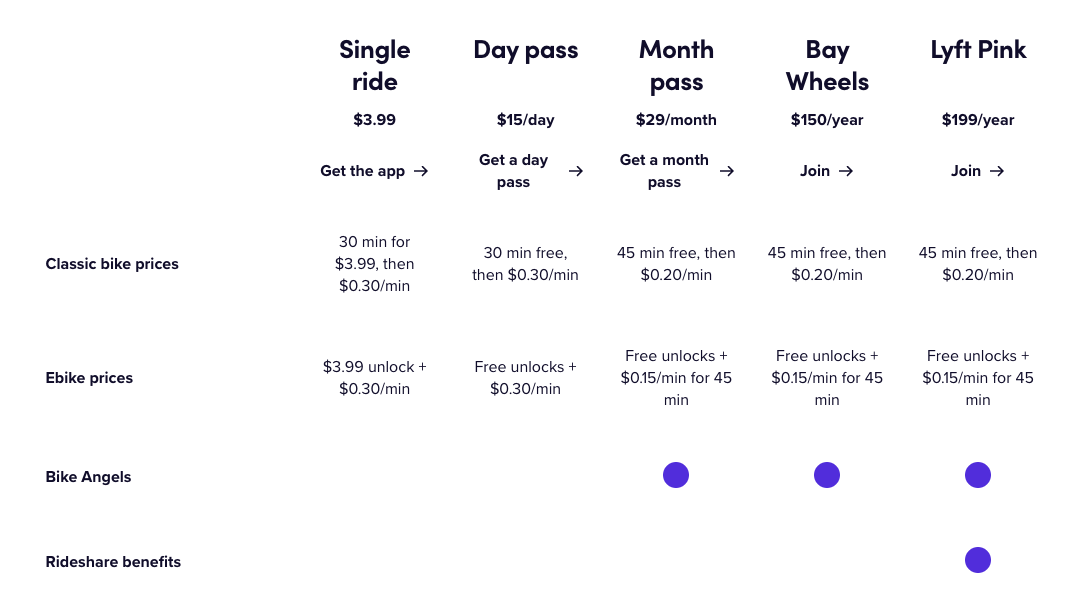
\includegraphics[width=1500px,height=500px]{BikeShareSubscription}

\small example of a subscription-based bike share service

\subsection{Introducing my Subject}\label{introducing-my-subject}


\includegraphics[width=250px,height=250px]{Cyclistic}


\includegraphics[width=250px,height=250px]{Divvy}

\subparagraph{My Data Analysis project will be on the fictional bike
share company Cyclistic, which is based on the real-life bike sharing
company Divvy, based in
Chicago.}\label{my-data-analysis-project-will-be-on-the-fictional-bike-share-company-cyclistic-which-is-based-on-the-real-life-bike-sharing-company-divvy-based-in-chicago.}

\subsubsection{Analysis Tools}\label{analysis-tools}

For this data analysis, I will be using:

\begin{enumerate}
\def\labelenumi{\arabic{enumi}.}
\tightlist
\item
  \href{sheets.google.com}{Google Sheets (Spreadsheet Editor)}
\item
  \href{https://posit.co/downloads/}{Posit's RStudio Cloud and RStudio
  Desktop}
\item
  R Markdown (To Produce this Summary)
\end{enumerate}

\subsection{Target Questions}\label{target-questions}

Based on the project specifications, this analysis will focus on
providing a answer and evidence to support these questions:

\begin{itemize}
\item ~
  \paragraph{How do annual members and casual riders use
  {[}Cyclistic/Divvy{]} bikes
  differently?}\label{how-do-annual-members-and-casual-riders-use-cyclisticdivvy-bikes-differently}
\item ~
  \paragraph{On average, would it be worth it for casual riders to
  upgrade to a annual subscription, and
  why?}\label{on-average-would-it-be-worth-it-for-casual-riders-to-upgrade-to-a-annual-subscription-and-why}
\end{itemize}

\subsection{\texorpdfstring{\textbf{Introducing the
Data}}{Introducing the Data}}\label{introducing-the-data}

We will be using publicly available comma-separated value data sheets
(DivvyQ12019.csv and DivvyQ12020.csv) available from
\href{https://divvybikes.com/system-data}{Divvy's data bank}. These two
spreadsheets contain Cyclistic's ridership data from 2019 Quarter 1 and
2020 Quarter 1. Specifically, for the first file Divvy\_Trips\_2019\_Q1
we are given the:

\begin{itemize}
\item
  Unique \textbf{trip\_id} of a bicycle trip (number)
\item
  \textbf{Start time and End time} of a trip (when a bicycle is taken
  out of a dock and put back in at the end), in ``year-month-day
  24-hour:minute:second'' format, sorted in ascending order by
  start\_time. (Datestamp)
\item
  Unique \textbf{id} of the bike that was used (Number)
\item
  Trip \textbf{duration} column between start time and end time, in
  seconds. (Number)
\item
  \textbf{Station which the bike was undocked at the beginning, and
  station which the bike was returned to at the end of the trip}, as
  well as \textbf{unique ids} of each station. (String)
\item
  \textbf{Status of the user of the bike} (Annual Subscriber or Casual
  rider) (String, either Subscriber or Customer)
\item
  Personal information of the user, including \textbf{gender} and
  \textbf{birth} \textbf{year}.
\end{itemize}

However, upon looking into Divvy\_Trips\_2020\_Q1, we are given similar
data, but the column names are inconsistent with the other file (we will
have to change this during data cleaning).

\begin{itemize}
\item
  Unique \textbf{ride\_id} of a bicycle trip (number)
\item
  \textbf{Rideable\_type} column (mostly docked\_bike in this case, but
  can also include docked\_scooter for E-scooter rentals) (String)
\item
  \textbf{Start time and End time} of a trip (when a bicycle is taken
  out of a dock and put back in at the end), in ``year-month-day
  24-hour:minute:second'' format, sorted in ascending order by
  start\_time. (Datestamp)
\item
  \textbf{Station} which the bike was undocked at the beginning, and
  station which the bike was returned to at the * end of the trip, as
  well as unique ids of each station. (String)
\item
  \textbf{Latitude and Longitude} of the start and end stations, which
  will not really be relevant in our case.
\item
  \textbf{Member\_casual}, which indicates if a rider is a subscribing
  customer or a casual rider.
\end{itemize}

This data is comprehensive, but contains a few errors we must correct
before starting the analysis process. To do so, we will import the data
into a spreadsheet software (I used Google Sheets) to get an idea of how
the data is organized, the quantity of the data, and remove visible
flaws which may skew the analysis.

\subsection{Cleaning with Google
Sheets}\label{cleaning-with-google-sheets}

To clean the provided excel/csv files of errors and other
irregularities, We will use Google Sheets to process it before loading
it into RStudio.

\begin{enumerate}
\def\labelenumi{\arabic{enumi}.}
\item
  \textbf{Remove all the blank cells from Birthdate and Gender,
  replacing them with N/A.}
\item
  Made sure all of the datestamps (Ride Start Time and Ride End Time)
  are accurate and in the correct format to analyze.
\item
  \textbf{Ensured that the Usertype column's data was binary,} since it
  could only have two possible values: Subscriber, or Customer
  (non-subscribed/casual rider). If another value appears, than it is a
  mistake and should be replaced with N/A.

  \includegraphics[width=7.60417in,height=\textheight]{https://lh7-rt.googleusercontent.com/docsz/AD_4nXf9esvSgBbrA05f1PTwEscS5WYvCy9kYK78GwaHzVkOytYRhDbxLFvVpV7WSpQbMRwI18Z2WUG_ri26hbvilH0LjmFFJCNs23j3-ALBBao5JpXiu4-1AZQP0EuEZop6GdL7HZqh?key=U0gznwBjKdVU-4EJ0aqtWVaH}
\item
  \textbf{Converted the TripDuration column into a easier-to-read time}
  (from seconds to ``hours:minutes:seconds'' format) in order to ensure
  accuracy throughout the whole process.
\item
  Used conditional formatting to \textbf{highlight the different status
  of the customers (blue/green for subscriber and orange for
  casual/non-subscribing customer).}
\item
  \textbf{Added a day\_of\_week column according to project's
  specifications,} which displays the day of the week in a
  easy-to-identify format (1 - Sunday, 7 - Saturday)
\end{enumerate}

\begin{center}\rule{0.5\linewidth}{0.5pt}\end{center}

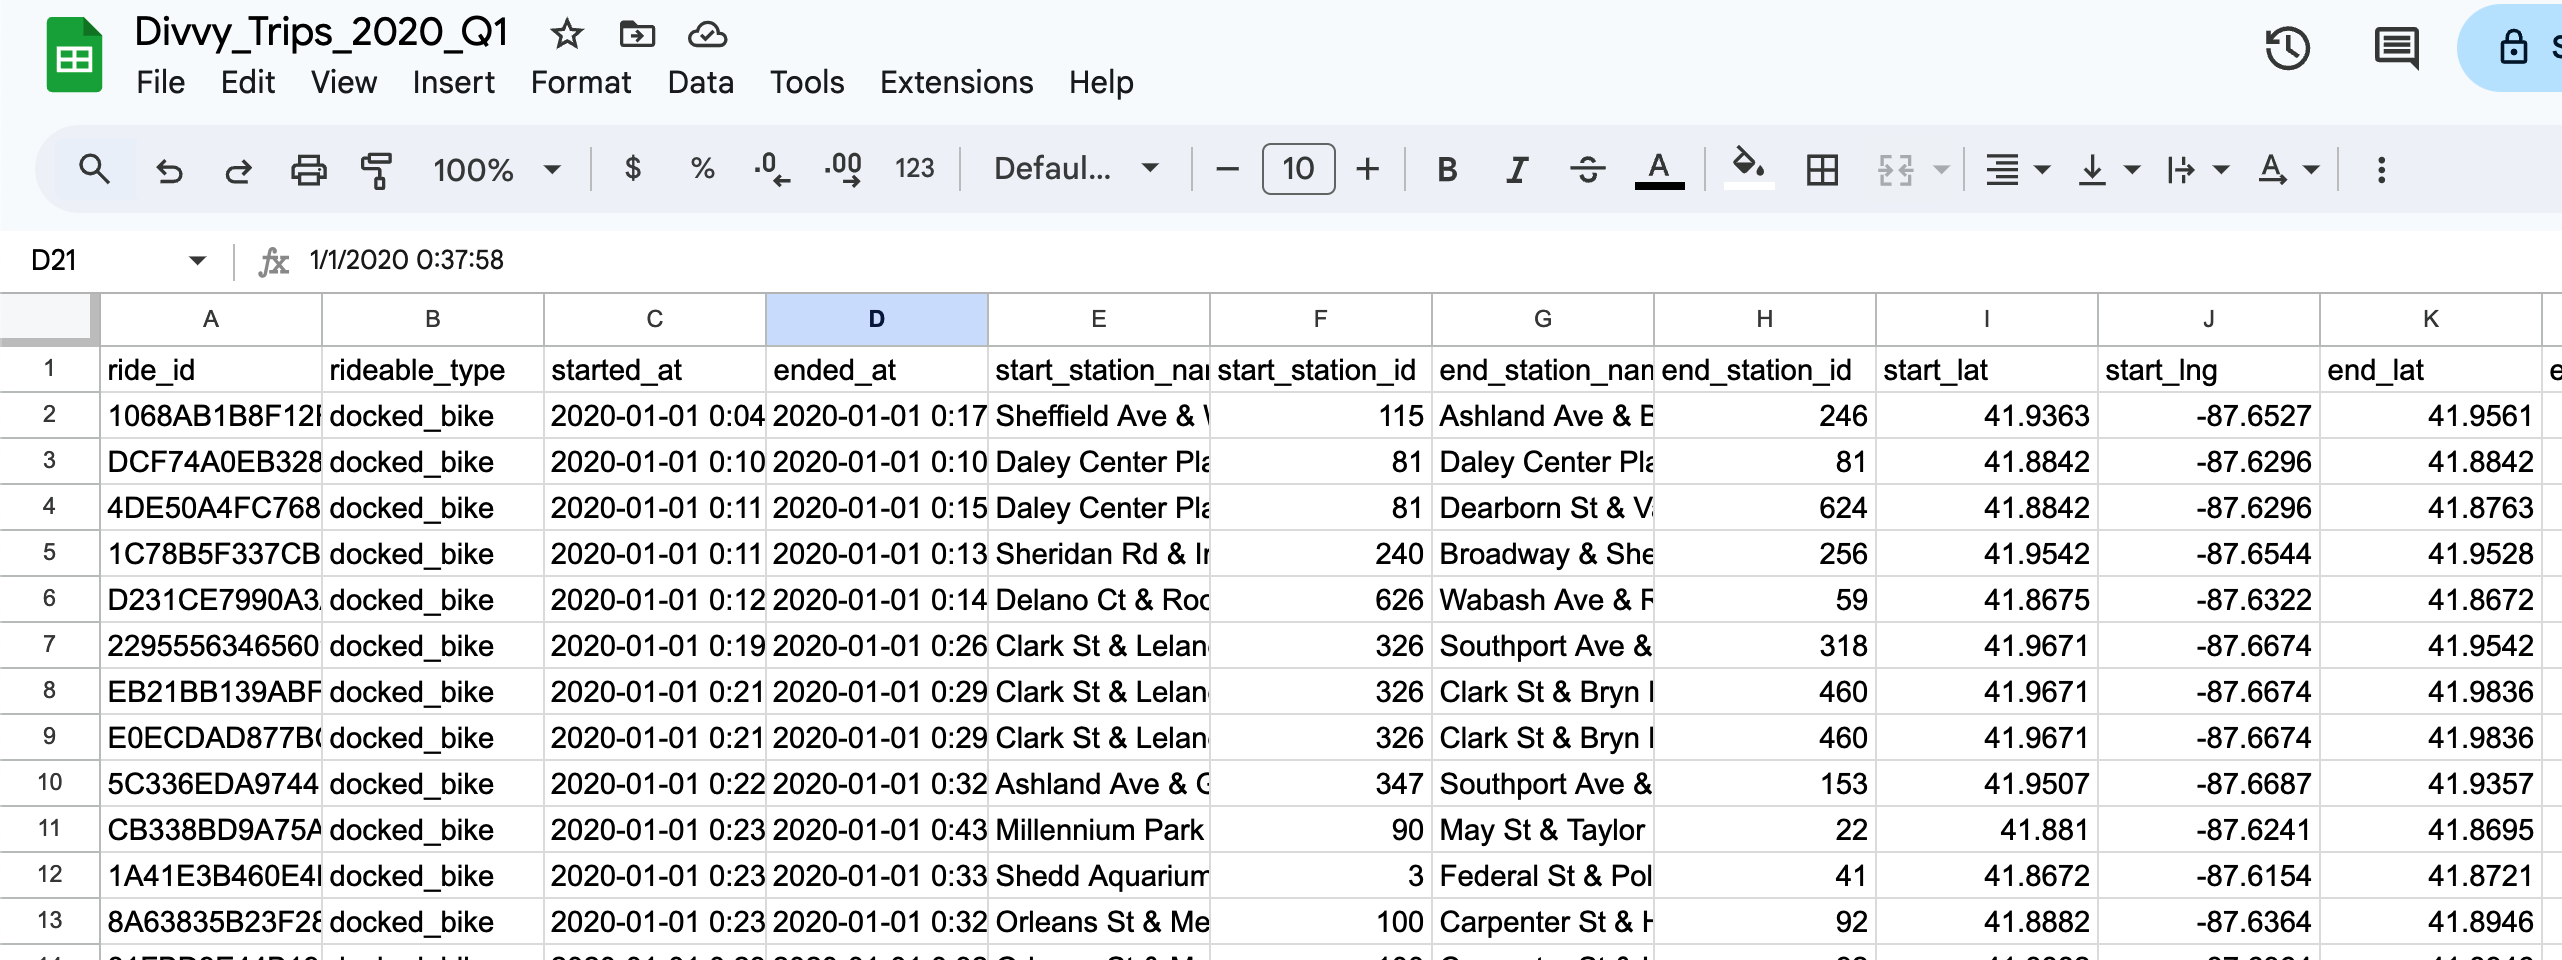
\includegraphics{images/Divvy_Trips_2020 Picture.png}

In addition, I also tried to make Divvy\_Trips\_2020\_Q1 consistent with
Divvy\_Trips\_2019\_Q1 by renaming some columns so they match the other
spreadsheet:

\begin{enumerate}
\def\labelenumi{\arabic{enumi}.}
\item
  \textbf{Renamed member\_casual to usertype,} and changed member to
  Subscriber, and casual to Customer.
\item
  \textbf{Added a ``tripDuration'' column as well as a ``ride\_length''
  column} with the same format as in the Q1 2019 spreadsheet.
\item
  \textbf{Added ``day\_of\_week''} column with start\_day represented as
  a day of the week (1 - Sunday, 7 - Saturday)
\item
  Checked for any blanks, and \textbf{replaced them with N/A}. (Wasn't
  fully effective, so I will have to do again in R)
\item
  Checked data for any improper values, and made sure all values matched
  their columns' appropriate datatypes.
\item
  \textbf{Sorted data by start\_time, in ascending order,} to match the
  format of Q1 2019 spreadsheet.
\end{enumerate}

\subsection{Deep Cleaning with R}\label{deep-cleaning-with-r}

\subsubsection{Setting up the
Environment}\label{setting-up-the-environment}

Before we start on R, we want to set up the environment and install all
necessary packages:

\begin{Shaded}
\begin{Highlighting}[]
\CommentTok{\#install.packages("tidyverse")}
\CommentTok{\#install.packages("dplyr")}
\CommentTok{\#install.packages("ggplot2")}

\CommentTok{\# Load in the packages}
\FunctionTok{library}\NormalTok{(tidyverse)}
\end{Highlighting}
\end{Shaded}

\begin{verbatim}
## -- Attaching core tidyverse packages ------------------------ tidyverse 2.0.0 --
## v dplyr     1.1.4     v readr     2.1.5
## v forcats   1.0.0     v stringr   1.5.1
## v ggplot2   3.5.1     v tibble    3.2.1
## v lubridate 1.9.4     v tidyr     1.3.1
## v purrr     1.0.4     
## -- Conflicts ------------------------------------------ tidyverse_conflicts() --
## x dplyr::filter() masks stats::filter()
## x dplyr::lag()    masks stats::lag()
## i Use the conflicted package (<http://conflicted.r-lib.org/>) to force all conflicts to become errors
\end{verbatim}

\begin{Shaded}
\begin{Highlighting}[]
\FunctionTok{library}\NormalTok{(dplyr)}
\FunctionTok{library}\NormalTok{(ggplot2)}
\end{Highlighting}
\end{Shaded}

Now that everything is installed, we can load our exported .csv files
into the editor, and familiarize ourselves with the data.

\begin{Shaded}
\begin{Highlighting}[]
\NormalTok{q1\_2019 }\OtherTok{\textless{}{-}} \FunctionTok{read\_csv}\NormalTok{(}\StringTok{"Divvy Trips Q1\_2019 (Cleaned).csv"}\NormalTok{) }\CommentTok{\#Assign variables}
\end{Highlighting}
\end{Shaded}

\begin{verbatim}
## Rows: 365069 Columns: 14
## -- Column specification --------------------------------------------------------
## Delimiter: ","
## chr  (7): start_time, end_time, from_station_name, to_station_name, usertype...
## dbl  (5): trip_id, bikeid, from_station_id, to_station_id, day_of_week
## num  (1): tripduration
## time (1): ride_length
## 
## i Use `spec()` to retrieve the full column specification for this data.
## i Specify the column types or set `show_col_types = FALSE` to quiet this message.
\end{verbatim}

\begin{Shaded}
\begin{Highlighting}[]
\NormalTok{q1\_2020 }\OtherTok{\textless{}{-}} \FunctionTok{read\_csv}\NormalTok{(}\StringTok{"Divvy Trips Q1\_2020 (Cleaned).csv"}\NormalTok{)}
\end{Highlighting}
\end{Shaded}

\begin{verbatim}
## Rows: 426887 Columns: 14
## -- Column specification --------------------------------------------------------
## Delimiter: ","
## chr  (7): ride_id, rideable_type, started_at, ended_at, start_station_name, ...
## dbl  (6): start_station_id, end_station_id, start_lat, start_lng, end_lat, e...
## time (1): ride_length
## 
## i Use `spec()` to retrieve the full column specification for this data.
## i Specify the column types or set `show_col_types = FALSE` to quiet this message.
\end{verbatim}

\begin{Shaded}
\begin{Highlighting}[]
\FunctionTok{colnames}\NormalTok{(q1\_2019) }\CommentTok{\#Find the column names and display them}
\end{Highlighting}
\end{Shaded}

\begin{verbatim}
##  [1] "trip_id"           "start_time"        "end_time"         
##  [4] "bikeid"            "tripduration"      "from_station_id"  
##  [7] "from_station_name" "to_station_id"     "to_station_name"  
## [10] "usertype"          "gender"            "birthyear"        
## [13] "ride_length"       "day_of_week"
\end{verbatim}

\begin{Shaded}
\begin{Highlighting}[]
\FunctionTok{colnames}\NormalTok{(q1\_2020)}
\end{Highlighting}
\end{Shaded}

\begin{verbatim}
##  [1] "ride_id"            "rideable_type"      "started_at"        
##  [4] "ended_at"           "start_station_name" "start_station_id"  
##  [7] "end_station_name"   "end_station_id"     "start_lat"         
## [10] "start_lng"          "end_lat"            "end_lng"           
## [13] "usertype"           "ride_length"
\end{verbatim}

From our column names output, we can see that the two csv files had
similar data, but different column names. In order to work on them in R,
we must change Q1 2019's column names to match up with the columns in Q1
2020's csv.

\begin{Shaded}
\begin{Highlighting}[]
\DocumentationTok{\#\# clean all of the data and make it consistent with q1\_2020}

\NormalTok{(q1\_2019 }\OtherTok{\textless{}{-}} \FunctionTok{rename}\NormalTok{(q1\_2019}
\NormalTok{                   ,}\AttributeTok{ride\_id =}\NormalTok{ trip\_id}
\NormalTok{                   ,}\AttributeTok{rideable\_type =}\NormalTok{ bikeid}
\NormalTok{                   ,}\AttributeTok{started\_at =}\NormalTok{ start\_time}
\NormalTok{                   ,}\AttributeTok{ended\_at =}\NormalTok{ end\_time}
\NormalTok{                   ,}\AttributeTok{start\_station\_name =}\NormalTok{ from\_station\_name}
\NormalTok{                   ,}\AttributeTok{start\_station\_id =}\NormalTok{ from\_station\_id}
\NormalTok{                   ,}\AttributeTok{end\_station\_name =}\NormalTok{ to\_station\_name}
\NormalTok{                   ,}\AttributeTok{end\_station\_id =}\NormalTok{ to\_station\_id}
\NormalTok{                   ,}\AttributeTok{member\_casual =}\NormalTok{ usertype}
\NormalTok{))}
\end{Highlighting}
\end{Shaded}

\begin{verbatim}
## # A tibble: 365,069 x 14
##     ride_id started_at      ended_at rideable_type tripduration start_station_id
##       <dbl> <chr>           <chr>            <dbl>        <dbl>            <dbl>
##  1 21742443 2019-01-01 0:0~ 2019-01~          2167          390              199
##  2 21742444 2019-01-01 0:0~ 2019-01~          4386          441               44
##  3 21742445 2019-01-01 0:1~ 2019-01~          1524          829               15
##  4 21742446 2019-01-01 0:1~ 2019-01~           252         1783              123
##  5 21742447 2019-01-01 0:1~ 2019-01~          1170          364              173
##  6 21742448 2019-01-01 0:1~ 2019-01~          2437          216               98
##  7 21742449 2019-01-01 0:1~ 2019-01~          2708          177               98
##  8 21742450 2019-01-01 0:1~ 2019-01~          2796          100              211
##  9 21742451 2019-01-01 0:1~ 2019-01~          6205         1727              150
## 10 21742452 2019-01-01 0:1~ 2019-01~          3939          336              268
## # i 365,059 more rows
## # i 8 more variables: start_station_name <chr>, end_station_id <dbl>,
## #   end_station_name <chr>, member_casual <chr>, gender <chr>, birthyear <chr>,
## #   ride_length <time>, day_of_week <dbl>
\end{verbatim}

\begin{Shaded}
\begin{Highlighting}[]
\NormalTok{q1\_2019 }\OtherTok{\textless{}{-}} \FunctionTok{mutate}\NormalTok{(q1\_2019, }\AttributeTok{ride\_id =} \FunctionTok{as.character}\NormalTok{(ride\_id)}
\NormalTok{                  ,}\AttributeTok{rideable\_type =} \FunctionTok{as.character}\NormalTok{(rideable\_type))}
\end{Highlighting}
\end{Shaded}

Now that everything matches up, we can combine our two data tables to
make everything easier to analyze and work with. We also want to change
some of the specific columns (like date, time, numbers) into their
appropriate formats so that R can process them correctly in sorting and
aggregation operations.

\begin{Shaded}
\begin{Highlighting}[]
\NormalTok{all\_trips }\OtherTok{\textless{}{-}} \FunctionTok{bind\_rows}\NormalTok{(q1\_2019, q1\_2020)}\CommentTok{\#, q3\_2019)\#, q4\_2019, q1\_2020)}

\NormalTok{all\_trips }\OtherTok{\textless{}{-}}\NormalTok{ all\_trips }\SpecialCharTok{\%\textgreater{}\%}
\FunctionTok{select}\NormalTok{(}\SpecialCharTok{{-}}\FunctionTok{c}\NormalTok{(start\_lat, start\_lng, end\_lat, end\_lng, birthyear, gender, }\StringTok{"tripduration"}\NormalTok{))}

\NormalTok{all\_trips }\OtherTok{\textless{}{-}}\NormalTok{ all\_trips }\SpecialCharTok{\%\textgreater{}\%}
  \FunctionTok{select}\NormalTok{(}\SpecialCharTok{{-}}\FunctionTok{c}\NormalTok{(day\_of\_week))}


\CommentTok{\# Add columns that list the date, month, day, and year of each ride}
\CommentTok{\# This will allow us to aggregate ride data for each month, day, or year ... before completing}
\CommentTok{\# https://www.statmethods.net/input/dates.html more on date formats in R found at that link}
\NormalTok{all\_trips}\SpecialCharTok{$}\NormalTok{date }\OtherTok{\textless{}{-}} \FunctionTok{as.Date}\NormalTok{(all\_trips}\SpecialCharTok{$}\NormalTok{started\_at) }\CommentTok{\#The default format is yyyy{-}mm{-}dd}
\NormalTok{all\_trips}\SpecialCharTok{$}\NormalTok{month }\OtherTok{\textless{}{-}} \FunctionTok{format}\NormalTok{(}\FunctionTok{as.Date}\NormalTok{(all\_trips}\SpecialCharTok{$}\NormalTok{date), }\StringTok{"\%m"}\NormalTok{)}
\NormalTok{all\_trips}\SpecialCharTok{$}\NormalTok{day }\OtherTok{\textless{}{-}} \FunctionTok{format}\NormalTok{(}\FunctionTok{as.Date}\NormalTok{(all\_trips}\SpecialCharTok{$}\NormalTok{date), }\StringTok{"\%d"}\NormalTok{)}
\NormalTok{all\_trips}\SpecialCharTok{$}\NormalTok{year }\OtherTok{\textless{}{-}} \FunctionTok{format}\NormalTok{(}\FunctionTok{as.Date}\NormalTok{(all\_trips}\SpecialCharTok{$}\NormalTok{date), }\StringTok{"\%Y"}\NormalTok{)}
\NormalTok{all\_trips}\SpecialCharTok{$}\NormalTok{day\_of\_week }\OtherTok{\textless{}{-}} \FunctionTok{format}\NormalTok{(}\FunctionTok{as.Date}\NormalTok{(all\_trips}\SpecialCharTok{$}\NormalTok{date), }\StringTok{"\%A"}\NormalTok{)}

\NormalTok{all\_trips}\SpecialCharTok{$}\NormalTok{ride\_length }\OtherTok{\textless{}{-}} \FunctionTok{difftime}\NormalTok{(all\_trips}\SpecialCharTok{$}\NormalTok{ended\_at,all\_trips}\SpecialCharTok{$}\NormalTok{started\_at)}

\NormalTok{all\_trips}\SpecialCharTok{$}\NormalTok{ride\_length }\OtherTok{\textless{}{-}} \FunctionTok{as.numeric}\NormalTok{(}\FunctionTok{as.character}\NormalTok{(all\_trips}\SpecialCharTok{$}\NormalTok{ride\_length))}
\end{Highlighting}
\end{Shaded}

Everything looks good so far. But, before we start analysis, lets make
sure that everything looks in order.

\begin{Shaded}
\begin{Highlighting}[]
\FunctionTok{nrow}\NormalTok{(all\_trips)}
\end{Highlighting}
\end{Shaded}

\begin{verbatim}
## [1] 791956
\end{verbatim}

\begin{Shaded}
\begin{Highlighting}[]
\FunctionTok{colnames}\NormalTok{(all\_trips)}
\end{Highlighting}
\end{Shaded}

\begin{verbatim}
##  [1] "ride_id"            "started_at"         "ended_at"          
##  [4] "rideable_type"      "start_station_id"   "start_station_name"
##  [7] "end_station_id"     "end_station_name"   "member_casual"     
## [10] "ride_length"        "usertype"           "date"              
## [13] "month"              "day"                "year"              
## [16] "day_of_week"
\end{verbatim}

\begin{Shaded}
\begin{Highlighting}[]
\FunctionTok{table}\NormalTok{(all\_trips}\SpecialCharTok{$}\NormalTok{member\_casual)}
\end{Highlighting}
\end{Shaded}

\begin{verbatim}
## 
##   Customer Subscriber 
##      23163     341906
\end{verbatim}

\begin{Shaded}
\begin{Highlighting}[]
\FunctionTok{summary}\NormalTok{(all\_trips}\SpecialCharTok{$}\NormalTok{ride\_length)}
\end{Highlighting}
\end{Shaded}

\begin{verbatim}
##     Min.  1st Qu.   Median     Mean  3rd Qu.     Max. 
##     -552      328      537     1184      910 10628422
\end{verbatim}

Notice that the ride\_length has a abnormally high maximum value of
10628422 seconds. That's about 123 days of riding a bike. This may have
happened if someone forgot to return the bike for a long time, or may
indicate a case of theft. However, in our data analysis, data points
like these will mess up our calculations by inflating the mean and
skewing the data towards the right. We can see this when we look at
quartile 1, the median, and quartile 3; \textbf{Since the mean is more
than double of the median, and more than quartile 3, we can see that
these abnormal data points have skewed this measure}.

Also, look at the minimum value of -552 seconds. This is also another
example of flawed data, since you can't ride a bike for negative five
minutes. So, before continuing, lets eliminate these data points and
other possibly flawed data points from our table.

\begin{Shaded}
\begin{Highlighting}[]
\DocumentationTok{\#\# Eliminate abnormally high ride\_lengths over 86,400 seconds (amount of time in a day)}
\DocumentationTok{\#\# Eliminate negative ride\_lengths and invalid station names }
\NormalTok{all\_trips\_v2 }\OtherTok{\textless{}{-}}\NormalTok{ all\_trips[}\SpecialCharTok{!}\NormalTok{(all\_trips}\SpecialCharTok{$}\NormalTok{ride\_length}\SpecialCharTok{\textgreater{}}\DecValTok{86400} \SpecialCharTok{|}\NormalTok{ all\_trips}\SpecialCharTok{$}\NormalTok{ride\_length}\SpecialCharTok{\textless{}}\DecValTok{0} \SpecialCharTok{|}\NormalTok{ all\_trips}\SpecialCharTok{$}\NormalTok{start\_station\_name }\SpecialCharTok{==} \StringTok{"HQ QR"}\NormalTok{),]}

\CommentTok{\# Should have done this earlier, but}
\CommentTok{\# remove rows if member\_casual is NA (data not available)}
\CommentTok{\# This should be okay since we still have over 200,000 data points for analysis}
\NormalTok{all\_trips\_v2 }\OtherTok{\textless{}{-}}\NormalTok{ all\_trips\_v2[}\SpecialCharTok{!}\NormalTok{(}\FunctionTok{is.na}\NormalTok{(all\_trips\_v2}\SpecialCharTok{$}\NormalTok{member\_casual)),]}
\CommentTok{\# Count number of customer and subscriber rides for future reference}
\NormalTok{number\_of\_customer\_rides }\OtherTok{\textless{}{-}}\NormalTok{ all\_trips\_v2 }\SpecialCharTok{\%\textgreater{}\%} 
  \FunctionTok{filter}\NormalTok{(all\_trips\_v2}\SpecialCharTok{$}\NormalTok{member\_casual }\SpecialCharTok{==} \StringTok{"Customer"}\NormalTok{) }\SpecialCharTok{\%\textgreater{}\%}
  \FunctionTok{nrow}\NormalTok{()}
\NormalTok{number\_of\_subscriber\_rides }\OtherTok{\textless{}{-}}\NormalTok{ all\_trips\_v2 }\SpecialCharTok{\%\textgreater{}\%} 
  \FunctionTok{filter}\NormalTok{(all\_trips\_v2}\SpecialCharTok{$}\NormalTok{member\_casual }\SpecialCharTok{==} \StringTok{"Subscriber"}\NormalTok{) }\SpecialCharTok{\%\textgreater{}\%}
  \FunctionTok{nrow}\NormalTok{()}

\FunctionTok{nrow}\NormalTok{(all\_trips\_v2)}
\end{Highlighting}
\end{Shaded}

\begin{verbatim}
## [1] 364877
\end{verbatim}

\begin{Shaded}
\begin{Highlighting}[]
\FunctionTok{summary}\NormalTok{(all\_trips\_v2}\SpecialCharTok{$}\NormalTok{ride\_length)}
\end{Highlighting}
\end{Shaded}

\begin{verbatim}
##    Min. 1st Qu.  Median    Mean 3rd Qu.    Max. 
##    61.0   326.0   524.0   769.5   865.0 85984.0
\end{verbatim}

After removing our flawed data points, our table still has over 300,000
rows, meaning that it has more than enough data to come up with a
accurate analysis and conclusion. Let's start analyzing in the next
step!

\subsection{Data Analysis Time}\label{data-analysis-time}

First, let's compare the average ride time between non-members
(customers) and subscribers by using the aggregate function for mean,
min, max, median, and standard deviation (measure of variability of data
points).

\begin{Shaded}
\begin{Highlighting}[]
\CommentTok{\# Get the Summary (Mean, Median, Maximum, Minimum and Standard Deviation) of our data}
\FunctionTok{aggregate}\NormalTok{(all\_trips\_v2}\SpecialCharTok{$}\NormalTok{ride\_length }\SpecialCharTok{\textasciitilde{}}\NormalTok{ all\_trips\_v2}\SpecialCharTok{$}\NormalTok{member\_casual, }\AttributeTok{FUN =}\NormalTok{ mean)}
\end{Highlighting}
\end{Shaded}

\begin{verbatim}
##   all_trips_v2$member_casual all_trips_v2$ride_length
## 1                   Customer                2116.8862
## 2                 Subscriber                 678.4683
\end{verbatim}

\begin{Shaded}
\begin{Highlighting}[]
\FunctionTok{aggregate}\NormalTok{(all\_trips\_v2}\SpecialCharTok{$}\NormalTok{ride\_length }\SpecialCharTok{\textasciitilde{}}\NormalTok{ all\_trips\_v2}\SpecialCharTok{$}\NormalTok{member\_casual, }\AttributeTok{FUN =}\NormalTok{ median)}
\end{Highlighting}
\end{Shaded}

\begin{verbatim}
##   all_trips_v2$member_casual all_trips_v2$ride_length
## 1                   Customer                     1396
## 2                 Subscriber                      501
\end{verbatim}

\begin{Shaded}
\begin{Highlighting}[]
\FunctionTok{aggregate}\NormalTok{(all\_trips\_v2}\SpecialCharTok{$}\NormalTok{ride\_length }\SpecialCharTok{\textasciitilde{}}\NormalTok{ all\_trips\_v2}\SpecialCharTok{$}\NormalTok{member\_casual, }\AttributeTok{FUN =}\NormalTok{ max)}
\end{Highlighting}
\end{Shaded}

\begin{verbatim}
##   all_trips_v2$member_casual all_trips_v2$ride_length
## 1                   Customer                    84589
## 2                 Subscriber                    85984
\end{verbatim}

\begin{Shaded}
\begin{Highlighting}[]
\FunctionTok{aggregate}\NormalTok{(all\_trips\_v2}\SpecialCharTok{$}\NormalTok{ride\_length }\SpecialCharTok{\textasciitilde{}}\NormalTok{ all\_trips\_v2}\SpecialCharTok{$}\NormalTok{member\_casual, }\AttributeTok{FUN =}\NormalTok{ min)}
\end{Highlighting}
\end{Shaded}

\begin{verbatim}
##   all_trips_v2$member_casual all_trips_v2$ride_length
## 1                   Customer                       61
## 2                 Subscriber                       61
\end{verbatim}

\begin{Shaded}
\begin{Highlighting}[]
\FunctionTok{aggregate}\NormalTok{(all\_trips\_v2}\SpecialCharTok{$}\NormalTok{ride\_length }\SpecialCharTok{\textasciitilde{}}\NormalTok{ all\_trips\_v2}\SpecialCharTok{$}\NormalTok{member\_casual, }\AttributeTok{FUN =}\NormalTok{ sd)}
\end{Highlighting}
\end{Shaded}

\begin{verbatim}
##   all_trips_v2$member_casual all_trips_v2$ride_length
## 1                   Customer                 3688.786
## 2                 Subscriber                 1332.295
\end{verbatim}

From this initial analysis, we can already tell a trend forming between
a rider's membership status and their average ride length. Based on what
we're seeing, it seems like \textbf{non-subscribers (casual customers)
From this analysis, we can see that Customers, while having less rides,
often ride their bikes longer than average compared to subscribers}.
This may be in part because of planned usage, where customers will use
Cyclistic's service if they really need to for longer trips, compared to
subscribers, who use it more casually and liberally.

However, before finalizing this, we must dig a bit deeper and look at
more of the data to make a informed decision. Next, let's analyze how
the day of the week will affect the average ride time for both
subscribing members and casual customers. We will use a more complex
multi-part pipe function to do this.

\begin{Shaded}
\begin{Highlighting}[]
\CommentTok{\# analyze ridership data by type and weekday. Sort by day of week and customer group}
\NormalTok{day\_of\_week\_vs\_avg\_duration }\OtherTok{\textless{}{-}}\NormalTok{ all\_trips\_v2 }\SpecialCharTok{\%\textgreater{}\%}
\FunctionTok{mutate}\NormalTok{(}\AttributeTok{weekday =} \FunctionTok{wday}\NormalTok{(started\_at, }\AttributeTok{label =} \ConstantTok{TRUE}\NormalTok{)) }\SpecialCharTok{\%\textgreater{}\%} 
\FunctionTok{group\_by}\NormalTok{(member\_casual, weekday) }\SpecialCharTok{\%\textgreater{}\%} 
\FunctionTok{summarise}\NormalTok{(}\AttributeTok{average\_duration =} \FunctionTok{mean}\NormalTok{(ride\_length)) }\SpecialCharTok{\%\textgreater{}\%} 
\FunctionTok{arrange}\NormalTok{(member\_casual, weekday)}
\end{Highlighting}
\end{Shaded}

\begin{verbatim}
## `summarise()` has grouped output by 'member_casual'. You can override using the
## `.groups` argument.
\end{verbatim}

\begin{Shaded}
\begin{Highlighting}[]
\NormalTok{day\_of\_week\_vs\_avg\_duration}
\end{Highlighting}
\end{Shaded}

\begin{verbatim}
## # A tibble: 14 x 3
## # Groups:   member_casual [2]
##    member_casual weekday average_duration
##    <chr>         <ord>              <dbl>
##  1 Customer      Sun                2114.
##  2 Customer      Mon                1912.
##  3 Customer      Tue                2184.
##  4 Customer      Wed                2082.
##  5 Customer      Thu                2042.
##  6 Customer      Fri                2028.
##  7 Customer      Sat                2254.
##  8 Subscriber    Sun                 713.
##  9 Subscriber    Mon                 664.
## 10 Subscriber    Tue                 677.
## 11 Subscriber    Wed                 667.
## 12 Subscriber    Thu                 658.
## 13 Subscriber    Fri                 667.
## 14 Subscriber    Sat                 764.
\end{verbatim}

From this, the trend repeats throughout all days of the week. So far, we
are inferring that from a per-distance point of view, non-subscribing
casual customers seem to have higher results independent of the day of
week.

Now, let's look at how the number of rides vary between the two groups,
according to day of the week. We will use the same function, except we
will add number of rides in the summarise function, which displays it
along with average duration.

\begin{Shaded}
\begin{Highlighting}[]
\CommentTok{\# analyze ridership data by type and weekday. Sort by day of week and customer group}
\NormalTok{day\_of\_week\_vs\_no\_rides }\OtherTok{\textless{}{-}}\NormalTok{ all\_trips\_v2 }\SpecialCharTok{\%\textgreater{}\%}
\FunctionTok{mutate}\NormalTok{(}\AttributeTok{weekday =} \FunctionTok{wday}\NormalTok{(started\_at, }\AttributeTok{label =} \ConstantTok{TRUE}\NormalTok{)) }\SpecialCharTok{\%\textgreater{}\%} 
\FunctionTok{group\_by}\NormalTok{(member\_casual, weekday) }\SpecialCharTok{\%\textgreater{}\%} 
\FunctionTok{summarise}\NormalTok{(}\AttributeTok{average\_duration =} \FunctionTok{mean}\NormalTok{(ride\_length), }\AttributeTok{number\_of\_rides =} \FunctionTok{n}\NormalTok{()) }\SpecialCharTok{\%\textgreater{}\%}  \CommentTok{\# added number\_of\_rides}
\FunctionTok{arrange}\NormalTok{(member\_casual, weekday)}
\end{Highlighting}
\end{Shaded}

\begin{verbatim}
## `summarise()` has grouped output by 'member_casual'. You can override using the
## `.groups` argument.
\end{verbatim}

\begin{Shaded}
\begin{Highlighting}[]
\NormalTok{day\_of\_week\_vs\_no\_rides}
\end{Highlighting}
\end{Shaded}

\begin{verbatim}
## # A tibble: 14 x 4
## # Groups:   member_casual [2]
##    member_casual weekday average_duration number_of_rides
##    <chr>         <ord>              <dbl>           <int>
##  1 Customer      Sun                2114.            3758
##  2 Customer      Mon                1912.            1887
##  3 Customer      Tue                2184.            2724
##  4 Customer      Wed                2082.            2482
##  5 Customer      Thu                2042.            2910
##  6 Customer      Fri                2028.            3363
##  7 Customer      Sat                2254.            5971
##  8 Subscriber    Sun                 713.           24219
##  9 Subscriber    Mon                 664.           48496
## 10 Subscriber    Tue                 677.           58254
## 11 Subscriber    Wed                 667.           57910
## 12 Subscriber    Thu                 658.           63962
## 13 Subscriber    Fri                 667.           59655
## 14 Subscriber    Sat                 764.           29286
\end{verbatim}

Now, let's display a summary of the max values from both of these tables

\begin{Shaded}
\begin{Highlighting}[]
\NormalTok{day\_of\_week\_vs\_avg\_duration }\SpecialCharTok{\%\textgreater{}\%}
  \FunctionTok{filter}\NormalTok{(average\_duration }\SpecialCharTok{==} \FunctionTok{max}\NormalTok{(average\_duration))}
\end{Highlighting}
\end{Shaded}

\begin{verbatim}
## # A tibble: 2 x 3
## # Groups:   member_casual [2]
##   member_casual weekday average_duration
##   <chr>         <ord>              <dbl>
## 1 Customer      Sat                2254.
## 2 Subscriber    Sat                 764.
\end{verbatim}

\begin{Shaded}
\begin{Highlighting}[]
\NormalTok{day\_of\_week\_vs\_no\_rides }\SpecialCharTok{\%\textgreater{}\%}
  \FunctionTok{filter}\NormalTok{(number\_of\_rides }\SpecialCharTok{==} \FunctionTok{max}\NormalTok{(number\_of\_rides))}
\end{Highlighting}
\end{Shaded}

\begin{verbatim}
## # A tibble: 2 x 4
## # Groups:   member_casual [2]
##   member_casual weekday average_duration number_of_rides
##   <chr>         <ord>              <dbl>           <int>
## 1 Customer      Sat                2254.            5971
## 2 Subscriber    Thu                 658.           63962
\end{verbatim}

\subsubsection{Graphical Representation}\label{graphical-representation}

We have the results of our analysis above. Here, we can see a different
pattern start to emerge, but just to make sure, let's create graphical
representations of these tables in the form of histograms.

\begin{Shaded}
\begin{Highlighting}[]
\NormalTok{all\_trips\_v2 }\SpecialCharTok{\%\textgreater{}\%}
  \FunctionTok{mutate}\NormalTok{(}\AttributeTok{weekday =} \FunctionTok{wday}\NormalTok{(started\_at, }\AttributeTok{label =} \ConstantTok{TRUE}\NormalTok{)) }\SpecialCharTok{\%\textgreater{}\%}
  \FunctionTok{group\_by}\NormalTok{(member\_casual, weekday) }\SpecialCharTok{\%\textgreater{}\%}
  
  \FunctionTok{summarise}\NormalTok{(}\AttributeTok{number\_of\_rides =} \FunctionTok{n}\NormalTok{()}
\NormalTok{            ,}\AttributeTok{average\_duration =} \FunctionTok{mean}\NormalTok{(ride\_length)) }\SpecialCharTok{\%\textgreater{}\%}
  \FunctionTok{arrange}\NormalTok{(member\_casual, weekday) }\SpecialCharTok{\%\textgreater{}\%}
  \FunctionTok{ggplot}\NormalTok{(}\FunctionTok{aes}\NormalTok{(}\AttributeTok{x =}\NormalTok{ weekday, }\AttributeTok{y =}\NormalTok{ number\_of\_rides, }\AttributeTok{fill =}\NormalTok{ member\_casual)) }\SpecialCharTok{+}
  \FunctionTok{labs}\NormalTok{(}\AttributeTok{title =} \StringTok{"Number of Rides vs. Day of the Week"}\NormalTok{,}
       \AttributeTok{caption=}\FunctionTok{paste0}\NormalTok{(}\StringTok{"Data from 2019 Q1 and 2020 Q1"}\NormalTok{)) }\SpecialCharTok{+}
  \FunctionTok{geom\_col}\NormalTok{(}\AttributeTok{position =} \StringTok{"dodge"}\NormalTok{)}
\end{Highlighting}
\end{Shaded}

\begin{verbatim}
## `summarise()` has grouped output by 'member_casual'. You can override using the
## `.groups` argument.
\end{verbatim}

\includegraphics{CyclisticAnalysisSummary_files/figure-latex/unnamed-chunk-15-1.pdf}

\begin{Shaded}
\begin{Highlighting}[]
\NormalTok{all\_trips\_v2 }\SpecialCharTok{\%\textgreater{}\%}
  \FunctionTok{mutate}\NormalTok{(}\AttributeTok{weekday =} \FunctionTok{wday}\NormalTok{(started\_at, }\AttributeTok{label =} \ConstantTok{TRUE}\NormalTok{)) }\SpecialCharTok{\%\textgreater{}\%}
  \FunctionTok{group\_by}\NormalTok{(member\_casual, weekday) }\SpecialCharTok{\%\textgreater{}\%}
  
  \FunctionTok{summarise}\NormalTok{(}\AttributeTok{number\_of\_rides =} \FunctionTok{n}\NormalTok{()}
\NormalTok{            ,}\AttributeTok{average\_duration =} \FunctionTok{mean}\NormalTok{(ride\_length)) }\SpecialCharTok{\%\textgreater{}\%}
  \FunctionTok{arrange}\NormalTok{(member\_casual, weekday) }\SpecialCharTok{\%\textgreater{}\%}
  \FunctionTok{ggplot}\NormalTok{(}\FunctionTok{aes}\NormalTok{(}\AttributeTok{x =}\NormalTok{ weekday, }\AttributeTok{y =}\NormalTok{ average\_duration, }\AttributeTok{fill =}\NormalTok{ member\_casual)) }\SpecialCharTok{+}
  \FunctionTok{labs}\NormalTok{(}\AttributeTok{title =} \StringTok{"Avg. Length of Ride vs. Day of the Week"}\NormalTok{,}
       \AttributeTok{caption=}\FunctionTok{paste0}\NormalTok{(}\StringTok{"Data from 2019 Q1 and 2020 Q1"}\NormalTok{)) }\SpecialCharTok{+}
  \FunctionTok{geom\_col}\NormalTok{(}\AttributeTok{position =} \StringTok{"dodge"}\NormalTok{)}
\end{Highlighting}
\end{Shaded}

\begin{verbatim}
## `summarise()` has grouped output by 'member_casual'. You can override using the
## `.groups` argument.
\end{verbatim}

\includegraphics{CyclisticAnalysisSummary_files/figure-latex/unnamed-chunk-16-1.pdf}

Upon looking in the graphs (especially the combined one), we can see the
trend identified above. Customers have higher average ride lengths
(about \textasciitilde2200 seconds or 36m, 40s) compared to subscribers
(about \textasciitilde700 seconds or 11m, 40s). This infers that
customers are on average likely to ride their Cyclistic bike almost 3x
the length as subscribers. Therefore, if the company wants to target
less consistent, butlonger-duration riders, they should focus on
attracting more non-subscribing customers. This will be beneficial if
Cyclistic bills per minute/timewise compared to upfront flat-rate.

On the other hand, the number of rides chart show that Subscribers have
a higher number of rides (almost 15 times more on peak days), while
having lower average ride times. Looking at Divvy's pricing strategy,
\textbf{this may be because of the perk ``45 minutes free'', which
includes free unlocks and complementary 45 minute riding time before a
charge of \$0.18 per minute}. So, taking this in account, these short
rides by subscribers would come at no cost on average, fueling
subscribers to take many more shorter distance rides, versus one longer
ride, which may start incurring fees once the time passes 2,700 seconds
(45 minutes).

\subsubsection{Taking a Deeper Dive on
Revenue}\label{taking-a-deeper-dive-on-revenue}

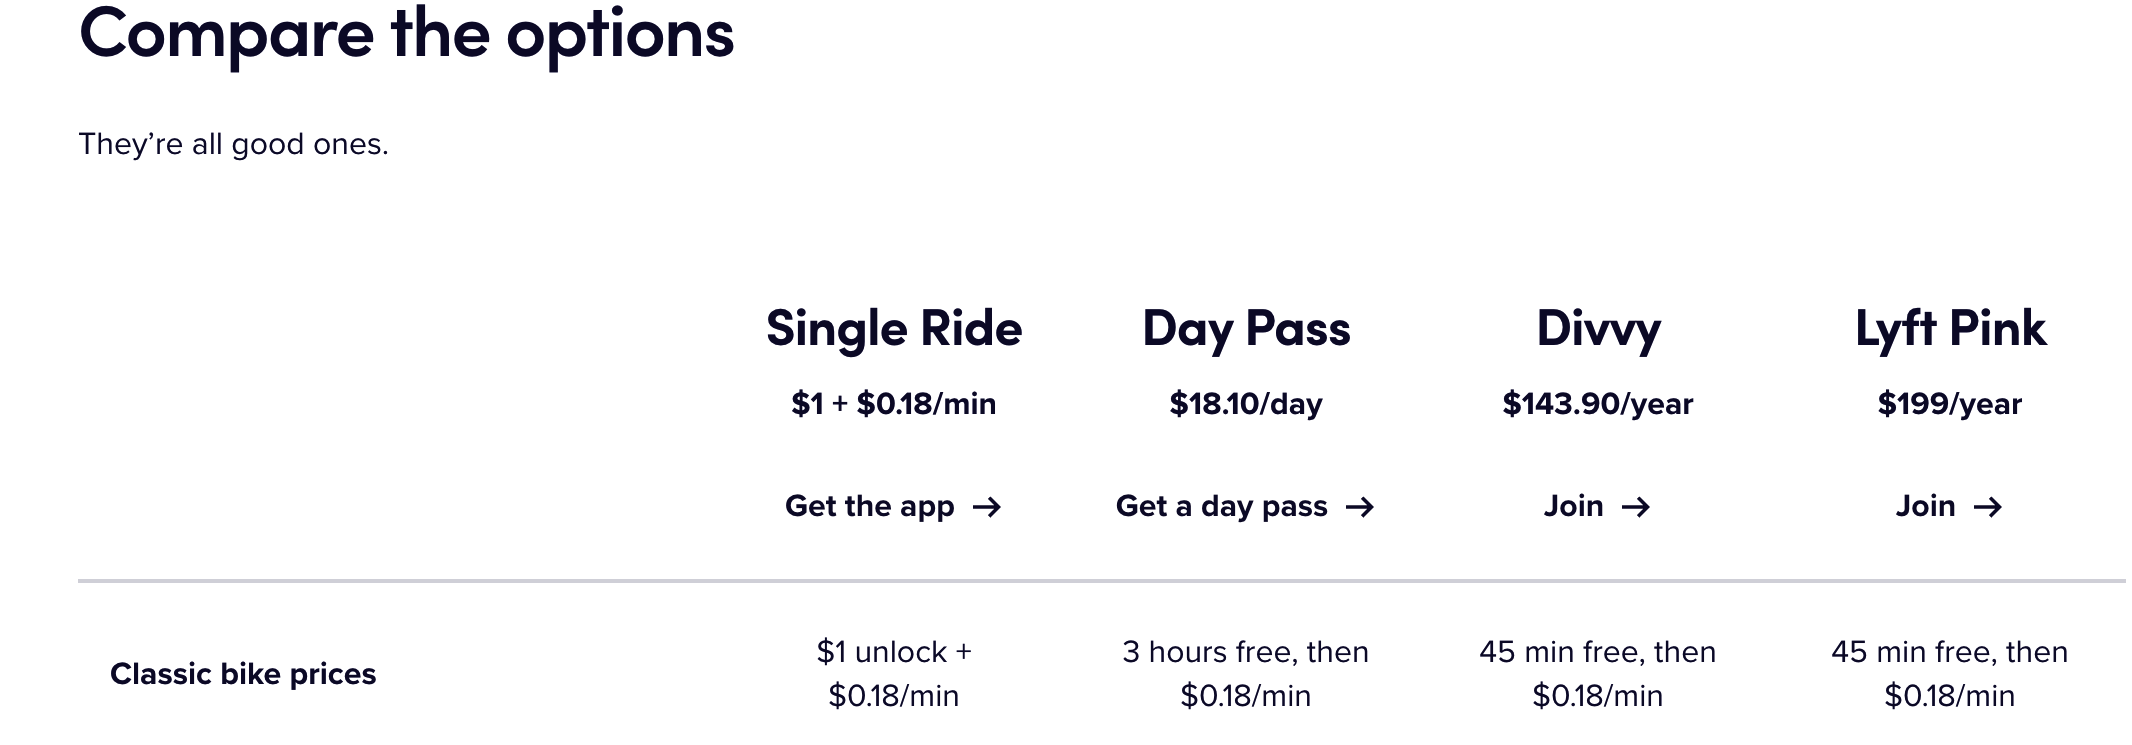
\includegraphics[width=1500px,height=300px]{Divvy Pricing}

Now, given the prices above, let's determine whether it is more
effective to try to attract customers to upgrade to annual subscribers.
Since the data source does not provide any personal identifiable
information (which allow us to distinguish the number of unique
subscribers to calculate profits from subscription fees), we will try to
compare the revenues of rides from subscribers and rides from customers.

First, let's find how much each ride from customers make on average:

\begin{Shaded}
\begin{Highlighting}[]
\CommentTok{\# $1 Unlock + $0.18 per minute}
\NormalTok{day\_of\_week\_vs\_no\_rides }\SpecialCharTok{\%\textgreater{}\%} 
  \FunctionTok{filter}\NormalTok{(member\_casual }\SpecialCharTok{==} \StringTok{"Customer"}\NormalTok{) }\SpecialCharTok{\%\textgreater{}\%} \CommentTok{\# Limit dataset to only customer rides}
  \FunctionTok{summarise}\NormalTok{(}\AttributeTok{revenue =} \DecValTok{1} \SpecialCharTok{+}\NormalTok{ (}\FloatTok{0.18} \SpecialCharTok{*}\NormalTok{ (average\_duration }\SpecialCharTok{/} \DecValTok{60}\NormalTok{))) }\CommentTok{\# Calculate average revenue per weekday}
\end{Highlighting}
\end{Shaded}

\begin{verbatim}
## Warning: Returning more (or less) than 1 row per `summarise()` group was deprecated in
## dplyr 1.1.0.
## i Please use `reframe()` instead.
## i When switching from `summarise()` to `reframe()`, remember that `reframe()`
##   always returns an ungrouped data frame and adjust accordingly.
## Call `lifecycle::last_lifecycle_warnings()` to see where this warning was
## generated.
\end{verbatim}

\begin{verbatim}
## `summarise()` has grouped output by 'member_casual'. You can override using the
## `.groups` argument.
\end{verbatim}

\begin{verbatim}
## # A tibble: 7 x 2
## # Groups:   member_casual [1]
##   member_casual revenue
##   <chr>           <dbl>
## 1 Customer         7.34
## 2 Customer         6.74
## 3 Customer         7.55
## 4 Customer         7.25
## 5 Customer         7.13
## 6 Customer         7.08
## 7 Customer         7.76
\end{verbatim}

The chunk of code calculated that the average revenue Divvy makes from
is around \$7.26 (\$6.74 to \$7.76). If we multiply this by the total
number of rides, we can get a rough average on how much Divvy earned
from customer rides during Q1 2019 and Q1 2020:

\begin{Shaded}
\begin{Highlighting}[]
\NormalTok{number\_of\_customer\_rides }\SpecialCharTok{*} \FloatTok{7.26}  \CommentTok{\# Multiply average customer revenue by number of customer rides}
\end{Highlighting}
\end{Shaded}

\begin{verbatim}
## [1] 167669.7
\end{verbatim}

\textbf{Around} \$\textbf{167,667.90} was made during these two
quarters. If we were to generalize and extend these results for a year,
\textbf{we find that \$335,339.40, or just under \$350,000 revenue was
generated from Divvy customer rides}. Relatively low, but this figure
makes sense because while each customer makes more money for the service
per ride, there are much fewer rides taken by customers than
subscribers.

Calculating the amount made from subscribers will be a bit more
time-consuming, since a lot of them rely on complementary rides which
are under 45 minutes, so, we will be working with all of the data rather
than just the average values.

\begin{Shaded}
\begin{Highlighting}[]
\CommentTok{\# Function to calculate revenue for subscribers:}
\CommentTok{\# If the time is under 45 minutes, free, otherwise, $0.18 per extra minute}
\NormalTok{subscriber\_revenue }\OtherTok{\textless{}{-}} \ControlFlowTok{function}\NormalTok{(duration)\{ }
  \ControlFlowTok{if}\NormalTok{(duration }\SpecialCharTok{\textless{}=}\NormalTok{ (}\DecValTok{45} \SpecialCharTok{*} \DecValTok{60}\NormalTok{))\{}
    \FunctionTok{return}\NormalTok{(}\DecValTok{0}\NormalTok{)}
\NormalTok{  \} }\ControlFlowTok{else}\NormalTok{ \{}
    \FunctionTok{return}\NormalTok{((}\FloatTok{0.18} \SpecialCharTok{*}\NormalTok{ ((duration }\SpecialCharTok{{-}}\NormalTok{ (}\DecValTok{45} \SpecialCharTok{*} \DecValTok{60}\NormalTok{)) }\SpecialCharTok{/} \DecValTok{60}\NormalTok{)))}
\NormalTok{  \}}
\NormalTok{\}}

\NormalTok{all\_trips\_v2 }\SpecialCharTok{\%\textgreater{}\%}
  \FunctionTok{filter}\NormalTok{(all\_trips\_v2}\SpecialCharTok{$}\NormalTok{member\_casual }\SpecialCharTok{==} \StringTok{"Subscriber"}\NormalTok{) }\SpecialCharTok{\%\textgreater{}\%} \CommentTok{\# Limit to only subscribers}
  \FunctionTok{mutate}\NormalTok{(}\AttributeTok{revenue =} \FunctionTok{sapply}\NormalTok{(ride\_length, subscriber\_revenue)) }\SpecialCharTok{\%\textgreater{}\%} \CommentTok{\# Calculate revenue for all rows}
  \FunctionTok{summarize}\NormalTok{(}\AttributeTok{total\_revenue =} \FunctionTok{sum}\NormalTok{(revenue)) }\CommentTok{\# Add everything up}
\end{Highlighting}
\end{Shaded}

\begin{verbatim}
## # A tibble: 1 x 1
##   total_revenue
##           <dbl>
## 1        39528.
\end{verbatim}

We will generalize and extend this data to cover a year by multiplying
it by two to get \$79,055. This may seem pretty low (since most members
take rides that are less than 45 minutes), but we must take into account
the membership amount. While data on this is not publicly available from
Divvy, a report from Chicago.gov states that Divvy annual membership
during 2020 can be estimated as around 30,715 people; So, with this in
account, we can estimate membership fees by multiplying membership cost
of \$143.90 / year by the amount of annual members which gets us
\$4,419,888.50. This all adds up to \textbf{\$4,498,943 total revenue
generated by annual members.}

\subsection{Conclusion and Next Steps}\label{conclusion-and-next-steps}


\includegraphics[width=600px,height=300px]{DivvyTruck}

\small A Divvy Truck next to a bike dock

Here's a recap about what we discovered during this data analysis
project:

\begin{longtable}[]{@{}
  >{\raggedright\arraybackslash}p{(\columnwidth - 4\tabcolsep) * \real{0.2167}}
  >{\raggedright\arraybackslash}p{(\columnwidth - 4\tabcolsep) * \real{0.1889}}
  >{\raggedright\arraybackslash}p{(\columnwidth - 4\tabcolsep) * \real{0.5889}}@{}}
\toprule\noalign{}
\begin{minipage}[b]{\linewidth}\raggedright
\end{minipage} & \begin{minipage}[b]{\linewidth}\raggedright
Customer
\end{minipage} & \begin{minipage}[b]{\linewidth}\raggedright
Subscribers
\end{minipage} \\
\midrule\noalign{}
\endhead
\bottomrule\noalign{}
\endlastfoot
Number of Rides & Low (23,095 for two quarters) & High (341,782 for two
quarters) \\
Average Ride Length & High (34.78 minutes) & Moderate-Low (10.97
minutes) \\
Revenue Generation from Rides & Average: \$7.26 per ride

Q1 2019 and 2020: \textbf{\$335,339}

Estimated Yearly: \textbf{\$670,668} & Average: \$0.11 per ride

Q1 2019 and 2020: \textbf{\$39,527}

Estimated Yearly: \textbf{\$79,054} \\
Revenue Generation from Subscription & \textbf{N/A}

\textbf{\$0} & Average: \$143.90 per year Estimated (based on
Chicago.gov data): \textbf{\$4,419,888.50} (\textasciitilde30,715
members) \\
\end{longtable}

\subsubsection{How do Subscribers and Customers Use Bikeshare
Differently?}\label{how-do-subscribers-and-customers-use-bikeshare-differently}

Our data has consistently shown that customers and subscribers use
Divvy/Cyclistic's services very differently; \textbf{Customers use the
service less often, but for longer amounts of time}, which generates
high profit per customer; however, the trade off is that many customers
only use the service a few times, and often only pay once or twice
through the year.

So, to appeal to customers while improving profits, the bike share
company should try to aim to upgrade them to paying subscribers; While
subscribers often ride for free, reducing individual ride revenues and
increasing wear from frequent bike use/docking, upgrading a customer
allows the company to collect \$143 in subscription revenue annually
(\textbf{which is almost worth 20 individual rides on average}).

\textbf{After paying a subscription fee, customers will receive the
ability to ride for free, motivating them to use the service more for
shorter distance trips;} As we have seen, our data supports this
conclusion, considering that subscribers ride fifteen times more often
than casual customers. \textbf{However, the ride length and the revenue
generated from per-minute/per-ride billing decreases}, considering that
despite a larger number of rides, subscribers collect about a tenth of
the revenue that regular customers collect.

\subsubsection{Are Subscriptions Worth the Money for
Customers?}\label{are-subscriptions-worth-the-money-for-customers}

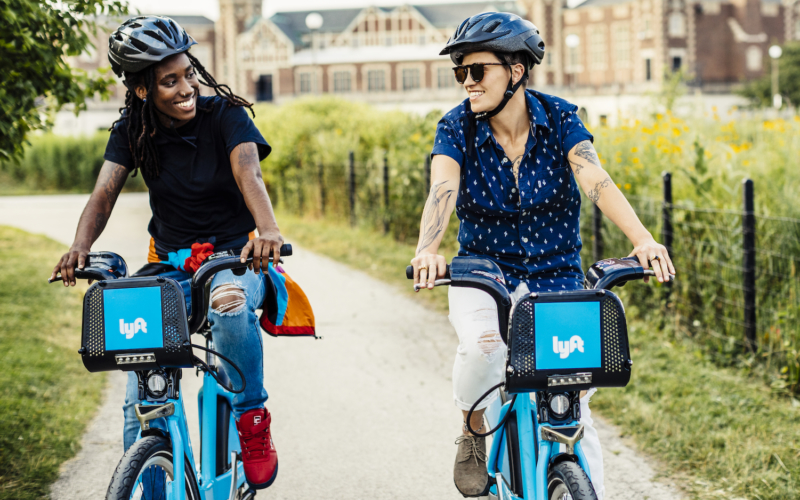
\includegraphics[width=700px,height=350px]{DivvyBikeImage}

It depends; If we look back on the data, we see that a annual
subscription pass is worth around 20 individual 35-minute rides. So, if
a customer is a more active user of the service, they would benefit from
getting the annual subscription because it will save them money in the
long run. If they use the service even more, they will get more out of
the subscription because it also provides them with extra benefits
similar to those provided with CitiBike's or Bay Wheel's subscription
plans.

However, since many of the customers only ride once or twice, it would
not be worth it for everyone to get the subscription. In that case,
appealing towards all riders would not be a good use of resources;
Cyclistic must appeal to the non-subscribing customers who rely on the
bikes the most, because they will be the most receptive to marketing
campaigns and in the end, will be more likely to convert from customer
to subscriber.

\subsubsection{Works Cited}\label{works-cited}

\begin{itemize}
\tightlist
\item
  \url{https://www.sciencedirect.com/science/article/abs/pii/S1366554523001345}
\item
  \url{https://www.lyft.com/bikes/bay-wheels/pricing}
\item
  \url{https://www.chicago.gov/city/en/depts/cdot/provdrs/bike/news/2023/april/divvy-for-the-entire-city--divvy-service-hits-all-50-wards.html}
\item
  \url{https://divvybikes.com/pricing}
\item
  \url{https://rstudio.github.io/cheatsheets/html/rmarkdown.html}
\end{itemize}

\end{document}
